%%%%%%%%%%%%%%%%%%%%%%%%%%%%%%%%%%%%%%%%%
% Proceedings of the National Academy of Sciences (PNAS)
% LaTeX Template
% Version 1.0 (19/5/13)
%
% This template has been downloaded from:
% http://www.LaTeXTemplates.com
%
% Original author:
% The PNAStwo class was created and is owned by PNAS:
% http://www.pnas.org/site/authors/LaTex.xhtml
% This template has been modified from the blank PNAS template to include
% examples of how to insert content and drastically change commenting. The
% structural integrity is maintained as in the original blank template.
%
% Original header:
%% PNAStmpl.tex
%% Template file to use for PNAS articles prepared in LaTeX
%% Version: Apr 14, 2008
%
%%%%%%%%%%%%%%%%%%%%%%%%%%%%%%%%%%%%%%%%%

%----------------------------------------------------------------------------------------
%	PACKAGES AND OTHER DOCUMENT CONFIGURATIONS
%----------------------------------------------------------------------------------------

%------------------------------------------------
% BASIC CLASS FILE
%------------------------------------------------

%% PNAStwo for two column articles is called by default.
%% Uncomment PNASone for single column articles. One column class
%% and style files are available upon request from pnas@nas.edu.

\documentclass[a4paper]{article}
%\documentclass{pnastwo}

%------------------------------------------------
% POSITION OF TEXT
%------------------------------------------------

%% Changing position of text on physical page:
%% Since not all printers position
%% the printed page in the same place on the physical page,
%% you can change the position yourself here, if you need to:

% \advance\voffset -.5in % Minus dimension will raise the printed page on the 
                         %  physical page; positive dimension will lower it.

%% You may set the dimension to the size that you need.

%------------------------------------------------
% GRAPHICS STYLE FILE
%------------------------------------------------

%% Requires graphics style file (graphicx.sty), used for inserting
%% .eps/image files into LaTeX articles.
%% Note that inclusion of .eps files is for your reference only;
%% when submitting to PNAS please submit figures separately.

%% Type into the square brackets the name of the driver program 
%% that you are using. If you don't know, try dvips, which is the
%% most common PC driver, or textures for the Mac. These are the options:

% [dvips], [xdvi], [dvipdf], [dvipdfm], [dvipdfmx], [pdftex], [dvipsone],
% [dviwindo], [emtex], [dviwin], [pctexps], [pctexwin], [pctexhp], [pctex32],
% [truetex], [tcidvi], [vtex], [oztex], [textures], [xetex]

\usepackage{graphicx}
%\usepackage{algorithmic}
%\usepackage{algorithm2e}


%------------------------------------------------
% ADDITIONAL OPTIONAL STYLE FILES
%------------------------------------------------

%% The AMS math files are commonly used to gain access to useful features
%% like extended math fonts and math commands.

\usepackage{amssymb,amsfonts,amsmath}

%------------------------------------------------
% OPTIONAL MACRO FILES
%------------------------------------------------

%% Insert self-defined macros here.
%% \newcommand definitions are recommended; \def definitions are supported

%\newcommand{\mfrac}[2]{\frac{\displaystyle #1}{\displaystyle #2}}
%\def\s{\sigma}


\begin{document}

%----------------------------------------------------------------------------------------
%	TITLE AND AUTHORS
%----------------------------------------------------------------------------------------

\title{Report on Machine Learning Lab, Ex 5} % For titles, only capitalize the first letter


\author{Mostafa Mohamed, Omar Kassem}%\affil{1}{Alberts-Ludwig Universt\"at Freiburg}}
%James Smith\affil{2}{University of Oregon}
%\and
%Jane Smith\affil{1}{}}

%\contributor{Submitted to Proceedings of the National Academy of Sciences of the United States of America}

%----------------------------------------------------------------------------------------

\maketitle % The \maketitle command is necessary to build the title page

%\begin{article}

%----------------------------------------------------------------------------------------
%	ABSTRACT, KEYWORDS AND ABBREVIATIONS
%----------------------------------------------------------------------------------------

%\begin{abstract}
%Abstract
%\end{abstract}

\section{Introduction}
This is a report about the deep learning lab, exercise 5. The general task of this assignment was extending assignment 3 to support new variants of the problem. The task of assignment 3 was to use Tensorflow/Keras to implement a convolutional neural network to train it on solving a search problem and compare it to the A* search algorithm.

\section{Search problem}
The given problem was find a target position in a given maze. We were given a simulator that can visualize our algorithm or the given reference A* algorithm. 
\subsection{Variation}
The variation of this problem that we attempt to solve in this assignment is solving the maze when the target position can change randomly across the map after each simulation.

\section{Architecture}
\begin{itemize}
\item Input: There was a given script that generates the train/validation data according to the A* algorithm. It starts from a variety of random positions and tries to search for the target. The A* reaches the target optimally.

\item Network: We used Keras to implement our neural network. We implemented a network that consists of 2 fully-connected layers followed by 3 convolutional layers. We tried different activation functions on some layers (like tanh), mostly the relu showed the best results.
\end{itemize}

\section{Approach}
We had 3 different ideas to change in order to attempt improving the results; namely 'knowing the destination', 'getting landmarks' and 'mark districts in the map'. The results we previously had was an accuracy of 31\% of solving the given map given that the target is changing randomly.
\subsection{Memorizing the target}
The idea here was to basically make the agent have an idea of how the target will be like while looking for it, the same idea is used in every day life, one needs to know how the destination is like before going in order to easily identify it.
We implement this by storing an extra state (along with the history of memorized states) of the local view of the target, and maintaining that it will always be identified as the target view.

\subsection{Coloring the walls}
Originally the colors of the wall was only red, but in more realistic examples we can often identify some landmarks of different regions, like the general architecture of buildings and so on.
Similarly here we start to color the walls depending on different regions. We had mainly 2 strategies for this coloring.
\begin{figure}
    \centerline{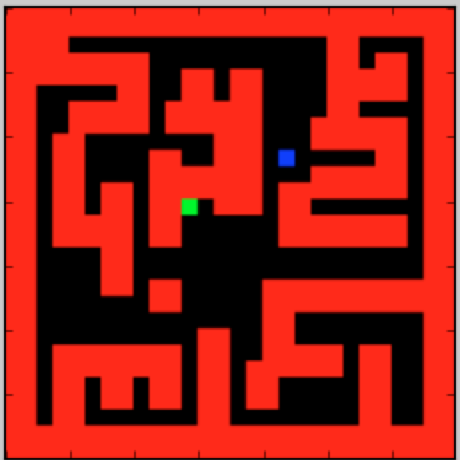
\includegraphics[width=0.30\linewidth]{problem.png}}
    \caption{Original maze}\label{fig1}
\end{figure}

\subsubsection{Simple coloring}
This approach divides the map into 4 equal regions, and colors each one of them with a different color.
\begin{figure}
    \centerline{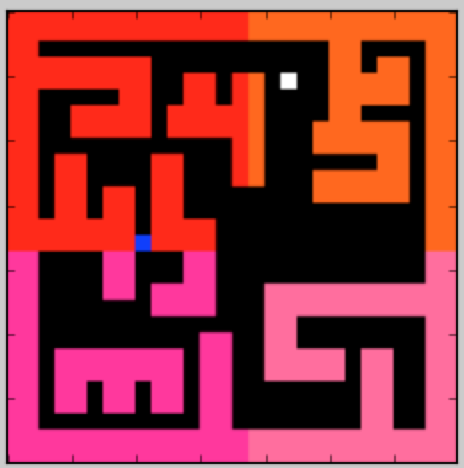
\includegraphics[width=0.35\linewidth]{simple.png}}
    \caption{Simple colouring} \label{fig2}
\end{figure}

\subsubsection{Gradient coloring}
This approach colors the walls by a gradient color (with a small random variation) with a gradient through out the diagonal of the map.

\begin{figure}
    \centerline{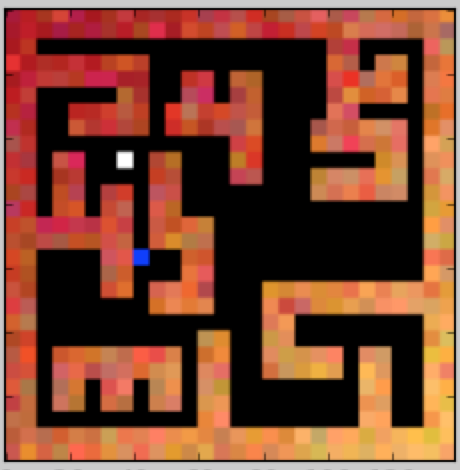
\includegraphics[width=0.35\linewidth]{gradient.png}}
    \caption{Gradient colouring} \label{fig3}
\end{figure}

\subsubsection{Some problems we faced}
\begin{itemize}
    \item We changed the color of the target to avoid confusion with other colors.
    \item We tried to avoid strong bluish colors for walls to avoid confusion with the bot.
    \item The colors of the walls are varying between reddish and yellowish colors.
\end{itemize}

\subsection{Gridding}
The idea here was to divide the map into a set of grids and instead of training the changing target randomly across the map.
We would make sure that each grid in the map is sampled equally. So that we don't end up knowing vacant areas more than tight areas.
We sample inside each grid either a representative of that grid (the middle element) with probability of 20\% or randomly from the grid otherwise. The combination of both will ensure that we "know" enough about the grid (even if we didn't reach the target exactly, we can still get close), and the randomization part in order not to be fixed on a specific place (thus missing {\it on purpose} potential targets while testing).

\subsubsection{Distance Accuracy}
In order to test that we got "close" enough to the target we computed (in addition to the already implemented accuracy) the distance accuracy.
It's computed by the formula $\frac{1}{1 + {\lfloor \frac{d}{g} \rfloor}^2}$, where $d$ is the distance between the bot and the target at the end of the game, and $g$ is the side length of the grid that we are using.

\section{Results}
We tried different combinations for the running. The girdding factor $g$ that we used is $3$ (Normal) or $6$ (Big).

\subsection{Standard map}
The map given in assignment 3, it's a $28 \times 28$ map, with a local view $5 \times 5$
We ran 8 experiments; for each we train 7 times and test 10 times for each of them, and these are the average results.
\begin{center}
    \begin{tabular}{| l | l | l | l | l |}
    \hline
    Target & Gridding & Color & Accuracy & Distance Accuracy \\ \hline
    No & No & No & 31\% & - \\ \hline
    Yes & No & No & 70\% & - \\ \hline
    Yes & No & Simple & 80\% & - \\ \hline
    Yes & No & Gradient & 66\% & - \\ \hline
    Yes & Yes & No & 70\% & 72\% \\ \hline
    Yes & Yes & Simple & 79\% & 81\% \\ \hline
    Yes & Big & Simple & 77\% & 82\% \\ \hline
    Yes & Big & Gradient & 64\% & 71\% \\ \hline
    \end{tabular}
\end{center}

\subsection{Big map}
A new map of size $50 \times 50$ with a local view of $9 \times 9$.
We ran 4 experiments; for each we train 2 times and test 10 times for each of them, and these are the average results.
The state size of this map was much bigger than the other maps which showed some restrictions while experimenting.
Unfortunately we couldn't run more experiments due to lack of resources: time, quota for saving tables and RAM memory for loading large tables.

\begin{figure}
    \centerline{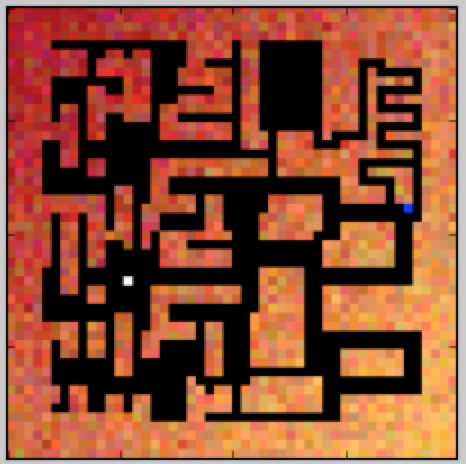
\includegraphics[width=0.45\linewidth]{bigmap.png}}
    \caption{Big Map}\label{fig4}
\end{figure}

\begin{center}
\begin{tabular}{| l | l | l | l | l |}
    \hline
    Target & Gridding & Color & Accuracy & Distance Accuracy \\ \hline
    No & No & No & 31\% & - \\ \hline
    Yes & No & Simple & 57\% & - \\ \hline
    Yes & Big& Simple & 62\% & 65\% \\ \hline
    Yes & Big & Gradient & 49\% & 55\% \\ \hline
    \end{tabular}
\end{center}

\subsection{Conclusion}
We can conclude from the experiments that memorizing the target showed a big improvement, further, the coloring of the walls (especially simple coloring), and finally for the big maps the gridding.


%----------------------------------------------------------------------------------------
%	FIGURES AND TABLES
%----------------------------------------------------------------------------------------

%% Adding Figure and Table References
%% Be sure to add figures and tables after \end{article}
%% and before \end{document}

%% For figures, put the caption below the illustration.
%%
%% \begin{figure}
%% \caption{Almost Sharp Front}\label{afoto}
%% \end{figure}
%% For Tables, put caption above table
%%
%% Table caption should start with a capital letter, continue with lower case
%% and not have a period at the end
%% Using @{\vrule height ?? depth ?? width0pt} in the tabular preamble will
%% keep that much space between every line in the table.

%% \begin{table}
%% \caption{Repeat length of longer allele by age of onset class}
%% \begin{tabular}{@{\vrule height 10.5pt depth4pt  width0pt}lrcccc}
%% table text
%% \end{tabular}
%% \end{table}

%% For two column figures and tables, use the following:

%% \begin{figure*}
%% \caption{Almost Sharp Front}\label{afoto}
%% \end{figure*}

%% \begin{table*}
%% \caption{Repeat length of longer allele by age of onset class}
%% \begin{tabular}{ccc}
%% table text
%% \end{tabular}
%% \end{table*}

%----------------------------------------------------------------------------------------

\end{document}
